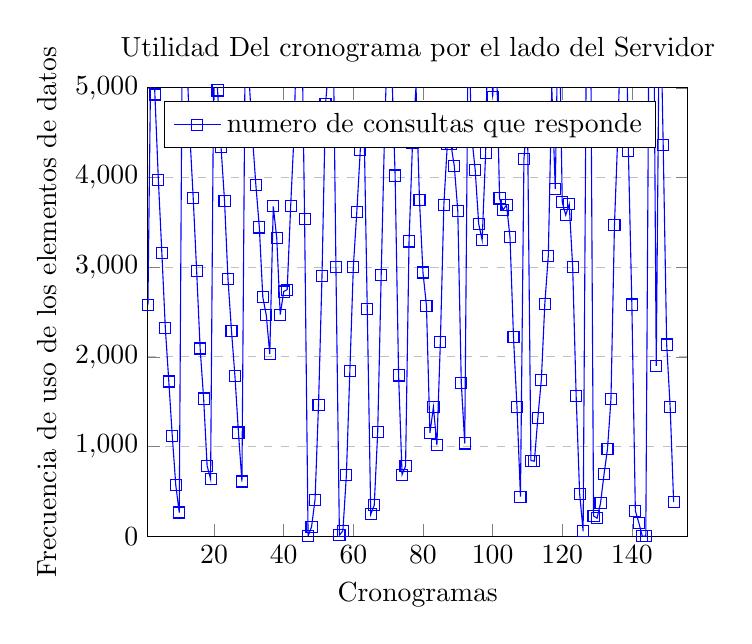
\begin{tikzpicture}
\begin{axis}[
    title={Utilidad Del cronograma por el lado del Servidor},
    xlabel={Cronogramas},
    ylabel={Frecuencia de uso de los elementos de datos},
    xmin=1, xmax=156,
    ymin=0, ymax=5000,
    xtick={},
    ytick={},
    legend pos=north west,
    ymajorgrids=true,
    grid style=dashed,
]

\addplot[
    color=blue,
    mark=square,
    ]
    coordinates {
%UTILIDAD TOTAL
(1,2577)
(2,5917)
(3,4926)
(4,3972)
(5,3160)
(6,2321)
(7,1725)
(8,1113)
(9,569)
(10,264)
(11,6540)
(12,5480)
(13,4509)
(14,3776)
(15,2953)
(16,2093)
(17,1535)
(18,785)
(19,637)
(20,5780)
(21,4971)
(22,4340)
(23,3742)
(24,2865)
(25,2290)
(26,1782)
(27,1156)
(28,610)
(29,5838)
(30,5140)
(31,4472)
(32,3918)
(33,3443)
(34,2666)
(35,2464)
(36,2031)
(37,3679)
(38,3325)
(39,2471)
(40,2728)
(41,2750)
(42,3681)
(43,4509)
(44,6108)
(45,6306)
(46,3540)
(47,2)
(48,104)
(49,408)
(50,1466)
(51,2904)
(52,4815)
(53,5287)
(54,6348)
(55,3002)
(56,11)
(57,60)
(58,680)
(59,1842)
(60,3005)
(61,3617)
(62,4307)
(63,4760)
(64,2530)
(65,244)
(66,345)
(67,1162)
(68,2913)
(69,4551)
(70,5760)
(71,5271)
(72,4022)
(73,1793)
(74,686)
(75,783)
(76,3287)
(77,4389)
(78,5014)
(79,3748)
(80,2941)
(81,2570)
(82,1151)
(83,1440)
(84,1016)
(85,2169)
(86,3698)
(87,4376)
(88,4378)
(89,4127)
(90,3629)
(91,1711)
(92,1034)
(93,5756)
(94,4460)
(95,4084)
(96,3484)
(97,3303)
(98,4275)
(99,6600)
(100,4894)
(101,5542)
(102,3767)
(103,3638)
(104,3693)
(105,3333)
(106,2221)
(107,1441)
(108,440)
(109,4204)
(110,4734)
(111,843)
(112,837)
(113,1322)
(114,1744)
(115,2593)
(116,3128)
(117,5002)
(118,3874)
(119,6224)
(120,3726)
(121,3582)
(122,3703)
(123,3004)
(124,1560)
(125,475)
(126,55)
(127,6008)
(128,6803)
(129,225)
(130,201)
(131,368)
(132,689)
(133,974)
(134,1530)
(135,3472)
(136,4512)
(137,5973)
(138,6669)
(139,4293)
(140,2583)
(141,284)
(142,149)
(143,0)
(144,0)
(145,6304)
(146,7647)
(147,1899)
(148,6392)
(149,4359)
(150,2137)
(151,1442)
(152,379)
    };
    \legend{numero de consultas que responde}

\end{axis}
\end{tikzpicture}

